\documentclass[sans,math-serif,solid,chem,code,notes,plot]{bmc}

% \titlehead{Bespoke Multipurpose Class}
\title{A Demonstration}
\subtitle{Of my BMC, created thanks to \LaTeX}
\author{tecosaur \footnotesize \\ Of Github}

\begin{document}

\maketitle{}
\fancytoc{}

\chapter{This is a Chapter}

\section{Content}
Lorem ipsum dolor sit amet, consectetur adipiscing elit. Mauris nec ante quis tellus aliquet fringilla id nec ligula. Pellentesque vulputate ligula in erat tincidunt, eu venenatis augue pellentesque. Vestibulum ante ipsum primis in faucibus orci luctus et ultrices posuere cubilia Curae; Sed a augue ut neque dignissim euismod ac nec augue. Pellentesque gravida congue elementum. Duis pulvinar pellentesque sodales. Sed pharetra, nibh nec gravida sagittis, sapien enim cursus diam, a iaculis tellus erat sit amet purus. Nunc tortor felis, ornare eu ultricies sit amet, ultrices vitae dui. Integer ac lacinia leo.\marginInfo[About this]{This is Lorem Ipsum}

\subsection{More content}
Cras eu sapien ut ipsum commodo placerat ac at diam. Aliquam suscipit urna nec condimentum iaculis. Duis hendrerit eros ac gravida tincidunt. Praesent orci odio, pulvinar sed metus ac, scelerisque tincidunt elit. Donec pharetra sit amet diam eu pellentesque. Praesent quis volutpat arcu. Aliquam auctor finibus vestibulum. Suspendisse accumsan porttitor neque, at tincidunt ex pharetra nec. Phasellus ac dolor eget nunc mattis ultricies. In et tellus vel magna accumsan varius eu nec leo. Curabitur odio dolor, porttitor in lectus sed, consequat consectetur elit. Morbi vel quam a elit mattis consequat ac vitae enim. Nullam condimentum turpis vel purus pretium, at viverra nibh gravida. Aenean quis enim ac mi euismod vehicula.

\infoInfo{Relevant Info}{In publishing and graphic design, lorem ipsum is a placeholder text used to demonstrate the visual form of a document without relying on meaningful content (also called \emph{greeking})}

\subsection{Another subsection}

Nam nec nisl tristique, pellentesque magna non, pretium nunc. Nunc non leo sapien. In hac habitasse platea dictumst. Cras laoreet augue lacus, nec cursus ante lobortis nec. Aliquam at neque ut quam consectetur hendrerit. Sed eu nibh at ipsum aliquam volutpat non ut mi. Integer sed tortor ut justo lobortis scelerisque. Nunc in gravida tortor, euismod tincidunt orci. Mauris euismod leo eget leo auctor, sed faucibus tellus gravida.

% \begin{CodeInfo}{Some code!}[Just a caption]
% 	\begin{CodeInfoLst}[python]
% #!/usr/bin/env python
% logfile = open("/var/log/syslog", "r")
% for line in logfile:
% 	line_split = line.split()
% 	print line_split
% 	list = line_split[0], line_split[1], line_split[2], line_split[4]
% 	print list
% 	\end{CodeInfoLst}
% 	Some info on the code
% \end{CodeInfo}

\section{Some Code}

\begin{minted}[highlightlines={3,10-11}]{python}
import numpy as np

 def incmatrix(genl1,genl2):
	m = len(genl1)
	n = len(genl2)
	M = None # to become the incidence matrix
	VT = np.zeros((n*m,1), int)  # dummy variable

	# compute the bitwise xor matrix ($\veebar$)
	M1 = bitxormatrix(genl1)
	M2 = np.triu(bitxormatrix(genl2),1)

	for i in range(m-1):
		for j in range(i+1, m):
			[r,c] = np.where(M2 == M1[i,j])
			for k in range(len(r)):
				VT[(i)*n + r[k]] = 1;
				VT[(i)*n + c[k]] = 1;
				VT[(j)*n + r[k]] = 1;
				VT[(j)*n + c[k]] = 1;

				if M is None:
					M = np.copy(VT)
				else:
					M = np.concatenate((M, VT), 1)

				VT = np.zeros((n*m,1), int)

	return M

print("this is a really long line, as far as lines go;  as such I fully expect it to be split onto a second line by minted")
\end{minted}

\newpage
\section{Some Maths}
\begin{align*}
	\Lap[e^{-at}\sin (\omega t)](s) & = \int_0^\infty e^{-st} e^{-at}\sin (\omega t) \, \dd t                                                                          \\
	\text{using }                   & \sin(\omega t) = \frac{1}{2i} \left( e^{i\omega t} - e^{-i\omega t} \right)                                                      \\
	                                & = \frac{1}{2i} \int_0^\infty e^{-st-at+i\omega t} - e^{-st-at-i\omega t} \, \dd t                                                \\
	                                & = \frac{1}{2i} {\left[ \frac{e^{-(s+a-i\omega)t}}{-(s+a-i\omega)} - \frac{e^{-(s+a+i\omega)t}}{-(s+a+i\omega)} \right]}_0^\infty \\
	\text{If } s > -a               & \implies -s-a < 0 \implies \lim_{t \to \infty}\cancelto{0}{e^{-(s+a\pm i\omega)t}} \text{ so,}                                   \\
	                                & = \frac{1}{2i} \left( \frac{1}{(s+a)-i\omega} - \frac{1}{(s+a)+i\omega} \right)                                                  \\
	                                & = \frac{\omega}{{(s+a)}^2+\omega^2}
\end{align*}
\questionInfo{I have some questions}{What even is a laplace transform? Why is the sky blue?}
\section{A Molecule or Two}
\chemfig{*6(-=-(-COOH)=-=)}
\chemfig{X-[1]=^[-1]-[1]-[-1]-[1]-[-1]=^[1]-[-1]}
\qquad
\chemfig{-[1](=[3]O)-[-1]}

\chapter{A Second Chapter}

\section{More Text}
\marginWarning*[Warning]{This paragraph has been reused.}
Nunc eros quam, scelerisque vel metus vitae, gravida dapibus tellus. Nunc tincidunt libero et faucibus cursus. Sed sed felis congue, pharetra quam non, gravida urna. Cras ultrices mattis justo sit amet porta. Praesent efficitur sed quam quis varius. Etiam non laoreet lorem, nec efficitur nunc. Nulla nunc nisi, aliquet ac tellus aliquet, auctor sagittis lectus. Quisque interdum mattis facilisis.

\section{Where Would We Be Without Lipsum?}

Lipsum is a scrambled latin text \url{https://en.wikipedia.org/wiki/Lorem_ipsum}. Praesent dapibus vulputate leo eu facilisis. Donec et libero felis. Etiam sollicitudin, odio non sodales lacinia, felis lacus porttitor diam, non hendrerit nisi quam sed lacus. Aliquam erat volutpat. Morbi nisi dui, scelerisque sit amet finibus sed, sollicitudin in erat. Maecenas ac viverra ante, eu malesuada neque. Mauris commodo nisl nec magna pulvinar ultrices. Lorem ipsum dolor sit amet, consectetur adipiscing elit.

\tipsInfo{A tip}{Is sometimes useful}

\newpage
Lorem ipsum dolor sit amet, consectetur adipiscing elit. Mauris nec ante quis tellus aliquet fringilla id nec ligula. Pellentesque vulputate ligula in erat tincidunt, eu venenatis augue pellentesque. Vestibulum ante ipsum primis in faucibus orci luctus et ultrices posuere cubilia Curae; Sed a augue ut neque dignissim euismod ac nec augue. Pellentesque gravida congue elementum. Duis pulvinar pellentesque sodales. Sed pharetra, nibh nec gravida sagittis, sapien enim cursus diam, a iaculis tellus erat sit amet purus. Nunc tortor felis, ornare eu ultricies sit amet, ultrices vitae dui. Integer ac lacinia leo.
\checkInfo{Check this}{Checking things can be a good idea}

\section{Sectioning}
This is an introduction to a section displaing different section commands
\subsection{A Demo}
More specificly this is a demo of \verb|section|, \verb|subsection|, \verb|subsubsection|, \verb|paragraph|, and \verb|subparagraph|.
\subsubsection{Now onto paragraphs}
Occasionaly one delves into the depth of paragraph and subparagraphs.
\paragraph{A Paragraph}
For instance this is a paragraph.
\subparagraph{A Subparagraph}
Sometimes, even a paragraph isn't deep enough.

\newpage
Lorem ipsum dolor sit amet, consectetur adipiscing elit. Mauris nec ante quis tellus aliquet fringilla id nec ligula. Pellentesque vulputate ligula in erat tincidunt, eu venenatis augue pellentesque. Vestibulum ante ipsum primis in faucibus orci luctus et ultrices posuere cubilia Curae; Sed a augue ut neque dignissim euismod ac nec augue. Pellentesque gravida congue elementum. Duis pulvinar pellentesque sodales. Sed pharetra, nibh nec gravida sagittis, sapien enim cursus diam, a iaculis tellus erat sit amet purus. Nunc tortor felis, ornare eu ultricies sit amet, ultrices vitae dui. Integer ac lacinia leo.

\begin{center}
	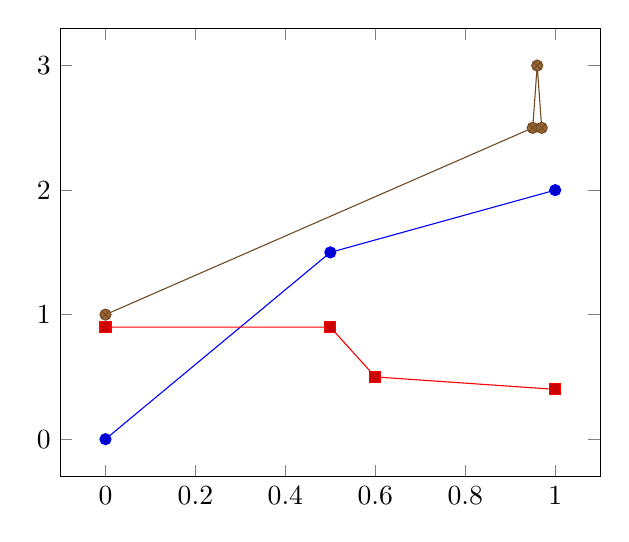
\begin{tikzpicture}
		\begin{axis}
		   \addplot coordinates{(0,0) (0.5,1.5) (1,2)};
		   \addplot coordinates{(0, 0.9) (0.5, 0.9) (0.6, 0.5) (1, 0.4)};
		   \addplot coordinates{(0,1) (0.95, 2.5) (0.96,3) (0.97,2.5)};
		\end{axis}
	 \end{tikzpicture}
\end{center}

 \criticalInfo{Big Issue}{Critical stuff needs to be paid attention to}

\newpage
Lorem ipsum dolor sit amet, consectetur adipiscing elit. Mauris nec ante quis tellus aliquet fringilla id nec ligula. Pellentesque vulputate ligula in erat tincidunt, eu venenatis augue pellentesque. Vestibulum ante ipsum primis in faucibus orci luctus et ultrices posuere cubilia Curae; Sed a augue ut neque dignissim euismod ac nec augue. Pellentesque gravida congue elementum. Duis pulvinar pellentesque sodales. Sed pharetra, nibh nec gravida sagittis, sapien enim cursus diam, a iaculis tellus erat sit amet purus. Nunc tortor felis, ornare eu ultricies sit amet, ultrices vitae dui. Integer ac lacinia leo.
\warningInfo{Hmm, this isn't the best}{Different lorem ipsum paragraphs would probably be better}

\chapter{A Third Chapter}

\end{document}
